\documentclass[11pt,a4paper]{article}
\usepackage[T1]{fontenc}
\usepackage[margin=2.3cm]{geometry}
\usepackage{amsmath,amssymb}
\usepackage{graphicx}
\usepackage[dvipsnames]{xcolor}
\usepackage{enumitem}
\usepackage[colorlinks=true,linkcolor=blue,urlcolor=blue]{hyperref}
\setlength{\parskip}{0.6em}
\setlength{\parindent}{0pt}
\begin{document}

\begin{center}{\LARGE\bfseries opengenetics}\\[0.4em]{\large Predict inheritance with Punnett squares, then watch genes drift and evolve.}\\[0.2em]\small PAN IIT OSS explainer \textbullet{} secondary school to diploma / undergraduate (levels 3-5)\end{center}

\section*{Why this exists}
Children inherit pairs of gene versions, and populations change over generations. This explainer shows the mathematics behind both, using only counting, probability and simple random sampling, so you can build it yourself.

\section*{The end goal}
Predict inheritance of traits with Punnett squares and simulation. The end goal is to predict inheritance of traits with Punnett squares and simulation, the starting toolkit of population genetics and of conservation biology. The same ideas of drift and selection appear in evolution, plant and animal breeding and in randomised algorithms.

\section*{How the three sessions build up}
\begin{enumerate}[nosep]
\item \textbf{Session 1: Genes in pairs and the Punnett square} (Level 1, conceptual interactive model, 60 min).
\item \textbf{Session 2: Probability, allele frequencies and Hardy-Weinberg} (Level 2, mathematical engineering model, 75 min).
\item \textbf{Session 3: Wright-Fisher simulation: drift, selection and mutation} (Level 3, simulation and validation, 90 min).
\end{enumerate}

\section{Session 1: Genes in pairs and the Punnett square}

\subsection*{A. Real-world problem}
Two parents both show the dominant trait, yet one of their children shows the recessive trait. Is that possible? A Punnett square answers it by listing every equally likely combination of alleles. This is a simplified textbook model of one gene; it is general education and says nothing about any real person or family, and it is not medical or genetic advice.

\subsection*{B. Concept and theory}
A gene can have versions called alleles. A child receives one allele from each parent, so each child has a pair. Write the dominant allele A and the recessive allele a. The genotype is the pair (AA, Aa or aa); the phenotype is the appearance. A dominant appearance needs at least one A; the recessive appearance needs aa. Each parent passes on one of their two alleles with equal chance 1/2. A Punnett square puts one parent's two alleles on the rows and the other's on the columns; its four boxes are the four equally likely children. For Aa x Aa the boxes are AA, Aa, Aa, aa, so genotypes are 1 : 2 : 1 and appearances are 3 dominant : 1 recessive.

\begin{itemize}[nosep]
\item A: dominant allele (no unit)
\item a: recessive allele (no unit)
\item genotype: the pair of alleles (AA, Aa, aa) (no unit)
\item phenotype: the visible trait: dominant or recessive (no unit)
\item n: number of children simulated (count)
\end{itemize}

\begin{equation*}
P(\text{child is } aa)=\tfrac12\times\tfrac12=\tfrac14
\end{equation*}

\begin{equation*}
\text{Aa}\times\text{Aa}:\quad AA:Aa:aa = 1:2:1,\qquad \text{dominant}:\text{recessive}=3:1
\end{equation*}

\begin{center}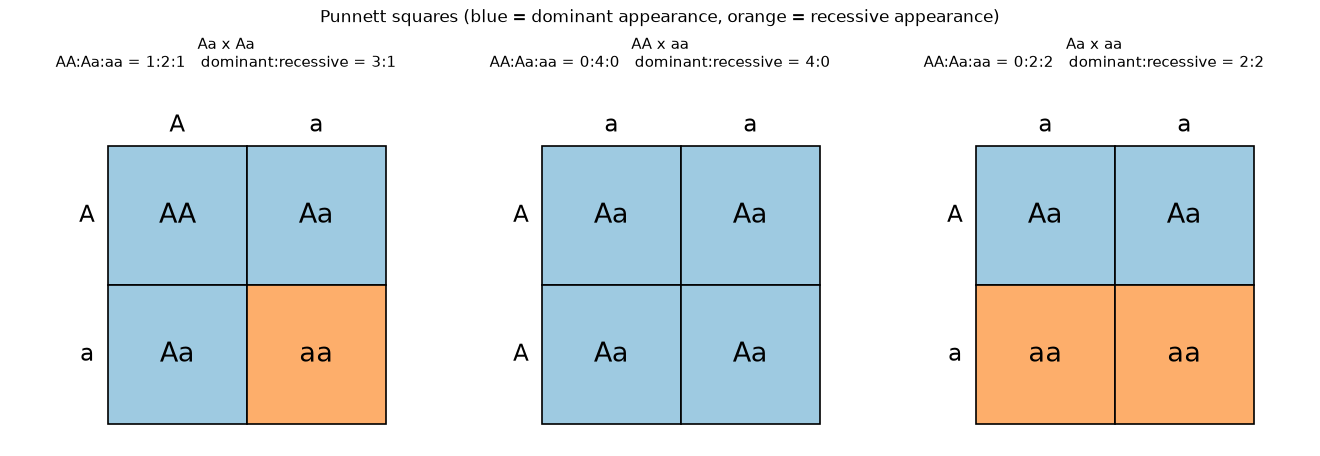
\includegraphics[width=0.85\linewidth]{figures/s01_punnett_squares.png}\\\small Three Punnett squares with genotype and appearance counts; blue boxes show the dominant appearance, orange the recessive.\end{center}

\subsection*{E. Worked example}
Both parents are Aa. List the possible children and state the genotype and appearance ratios.
\begin{enumerate}[nosep]
\item Parent 1 can pass A or a; parent 2 can pass A or a. Put them on the rows and columns.
\item The four boxes are AA, Aa, aA (written Aa) and aa.
\item Genotype counts: AA 1, Aa 2, aa 1, so the ratio is 1 : 2 : 1.
\item Appearance: AA and both Aa show the dominant trait (3 boxes); only aa shows the recessive trait (1 box), so the ratio is 3 : 1.
\item Each box has probability 1/4, so each child has probability 1/4 of being aa.
\end{enumerate}
\textbf{Answer.} Genotypes 1 AA : 2 Aa : 1 aa; appearance 3 dominant : 1 recessive; P(aa) = 1/4 for each child.

\subsection*{F. Questions}
\begin{enumerate}[nosep]
\item \textbf{Conceptual.} Two parents both show the dominant trait and have a child with the recessive trait. What must the genotypes of the parents be? Why?
\item \textbf{Numerical.} For the cross AA x Aa, fill in the Punnett square and give the genotype counts and the chance that a child shows the recessive appearance.
\item \textbf{Graph and simulation interpretation.} In the second figure, why does the fraction of recessive children jump around for 10 children but sit close to 1/4 for 10000?
\item \textbf{Design and optimisation challenge.} Design: you cross two plants and want about half of the offspring to show the recessive appearance. Which parent genotypes would you choose, and why not the other choices?
\end{enumerate}

\section{Session 2: Probability, allele frequencies and Hardy-Weinberg}

\subsection*{A. Real-world problem}
A recessive trait appears in about 1 birth in 10,000. How many people carry one copy of the allele without showing the trait? Counting boxes in a Punnett square no longer helps, because the parents are not chosen: we need the frequency of each allele in a whole population. And when a breeder counts offspring, how far from 3 : 1 is too far? General education in an idealised model; it is not medical or genetic advice about any person.

\subsection*{B. Concept and theory}
The rules are the ones from coin flips. Multiplication rule: for independent events, P(first and second) = P(first) x P(second). Addition rule: for events that cannot both happen, P(first or second) = P(first) + P(second). In Aa x Aa each parent passes a with probability 1/2, so P(aa) = 1/2 x 1/2 = 1/4, and P(Aa) = 1/4 + 1/4 = 1/2 (A from parent 1 and a from parent 2, or the other way round). In a population let p be the fraction of all alleles that are A and q the fraction that are a; then p + q = 1. If mating is random, there is no selection, no migration, no mutation and the population is large, the genotype proportions are p\textasciicircum{}2 (AA), 2pq (Aa) and q\textasciicircum{}2 (aa), and they add to (p + q)\textasciicircum{}2 = 1. This is the Hardy-Weinberg model, a baseline to compare real populations against. For a recessive trait seen in a fraction r of births, q = sqrt(r). To test counts against a 3:1 ratio, compute chi-square = sum of (observed - expected)\textasciicircum{}2 / expected; for two categories (1 degree of freedom) the standard table value for the 5 percent level is 3.84, and a larger statistic means the 3 : 1 ratio is doubted. For two genes inherited independently multiply the single-gene ratios: (3 : 1) x (3 : 1) = 9 : 3 : 3 : 1.

\begin{itemize}[nosep]
\item p: frequency of allele A (no unit (0 to 1))
\item q: frequency of allele a (no unit (0 to 1))
\item r: frequency of the recessive appearance (aa) (no unit)
\item O, E: observed and expected counts in a category (count)
\item chi2: chi-square statistic (no unit)
\item n: number of offspring counted (count)
\end{itemize}

\begin{equation*}
P(A\text{ and }B)=P(A)P(B),\qquad P(A\text{ or }B)=P(A)+P(B)\ \ (\text{exclusive})
\end{equation*}

\begin{equation*}
p+q=1,\qquad p^2+2pq+q^2=(p+q)^2=1
\end{equation*}

\begin{equation*}
q=\sqrt{r},\qquad \text{carriers}=2pq
\end{equation*}

\begin{equation*}
\hat q=\frac{2n_{aa}+n_{Aa}}{2\,(n_{AA}+n_{Aa}+n_{aa})}
\end{equation*}

\begin{equation*}
\chi^2=\sum\frac{(O-E)^2}{E},\qquad \chi^2<3.84\ \Rightarrow\ \text{3:1 not rejected at the 5\% level}
\end{equation*}

\begin{center}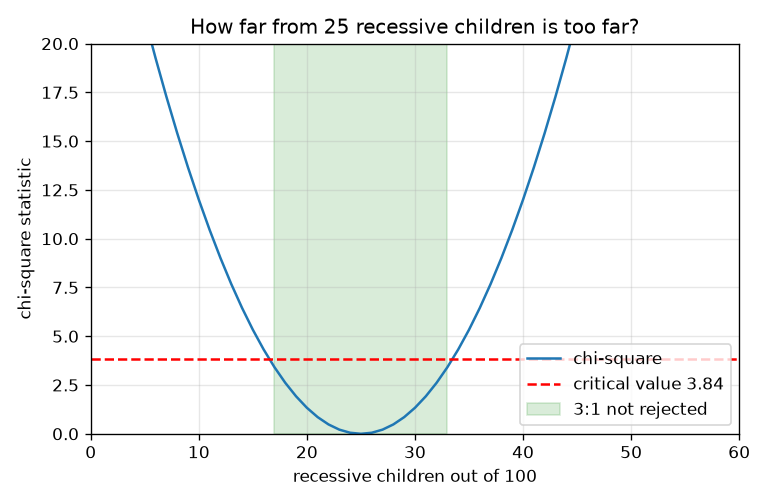
\includegraphics[width=0.85\linewidth]{figures/s02_chi_square_100.png}\\\small Chi-square against the recessive count out of 100: below 3.84 for 17 to 33 recessive children.\end{center}

\subsection*{E. Worked example}
A recessive trait is present in 1 birth in 10,000. Find q, p and the carrier proportion 2pq.
\begin{enumerate}[nosep]
\item q\textasciicircum{}2 = 1 / 10,000 = 0.0001.
\item q = sqrt(0.0001) = 0.01, so p = 1 - 0.01 = 0.99.
\item Carriers: 2pq = 2 x 0.99 x 0.01 = 0.0198.
\item 1 / 0.0198 is about 50, so roughly 1 person in 50 carries one copy, although only 1 in 10,000 shows the trait.
\item Check: p\textasciicircum{}2 + 2pq + q\textasciicircum{}2 = 0.9801 + 0.0198 + 0.0001 = 1.
\end{enumerate}
\textbf{Answer.} q = 0.01, p = 0.99 and carriers 2pq = 0.0198 (about 1 in 50). Most copies of a rare recessive allele are hidden in carriers.

\subsection*{F. Questions}
\begin{enumerate}[nosep]
\item \textbf{Conceptual.} Why do most copies of a rare recessive allele sit in carriers (Aa) rather than in people showing the trait (aa)?
\item \textbf{Numerical.} A recessive trait has frequency 1 in 2,500. Find q and the carrier proportion. Sanity check the result.
\item \textbf{Graph and simulation interpretation.} In the chi-square graph for 100 children, what range of recessive counts keeps the 3:1 ratio, and why is the curve lowest at 25?
\item \textbf{Design and optimisation challenge.} Design: a breeder counts 740 dominant and 260 recessive offspring of 1000 and suspects 3:1. Test it. Then say what range of recessive counts out of 1000 would be accepted, and why a bigger sample is a stronger test.
\end{enumerate}

\section{Session 3: Wright-Fisher simulation: drift, selection and mutation}

\subsection*{A. Real-world problem}
In a small population a gene version can vanish, or take over, purely by luck, even if it helps survival. In a large population the same helpful version spreads steadily. How small is too small, and how large must a captive breeding population be to keep most of its genetic variety for 50 generations? This is an idealised classroom model for general education. It is not a tool for real conservation decisions and says nothing about any person.

\subsection*{B. Concept and theory}
Wright-Fisher model: N diploid individuals carry 2N alleles. Each generation does three steps: selection and mutation change the expected frequency, then random mating draws the next 2N alleles independently, so the number of A alleles is Binomial(2N, p) and the new frequency is that number divided by 2N. That random sampling is genetic drift: it has no direction but changes frequencies by about sqrt(p q / (2N)) per generation, so small populations drift faster. Heterozygosity H = 2pq falls on average by the factor (1 - 1/(2N)) each generation, so E[H\_t] = H\_0 (1 - 1/(2N))\textasciicircum{}t. A neutral allele at frequency p\_0 eventually takes over (fixes) with probability p\_0 and is lost with probability 1 - p\_0. Selection: fitness of AA, Aa, aa is 1 + s, 1 + h s, 1; the update is p' = [p\textasciicircum{}2 (1 + s) + p q (1 + h s)] / wbar with mean fitness wbar = p\textasciicircum{}2 (1 + s) + 2 p q (1 + h s) + q\textasciicircum{}2 (h = 1/2 additive, h = 1 dominant advantage, h = 0 recessive advantage). A simple haploid-like advantage uses p' = p (1 + s) / (1 + s p), whose closed form is logit(p\_t) = logit(p\_0) + t ln(1 + s). Mutation as a small constant flow: p' = p (1 - mu) + (1 - p) nu, settling at p* = nu / (mu + nu). In the simulation each generation applies selection, then mutation, then drift.

\begin{itemize}[nosep]
\item N: number of diploid individuals (count)
\item p, q: frequency of A and a (p + q = 1) (no unit)
\item s: fitness advantage of A (no unit)
\item h: dominance of the advantage (0 to 1) (no unit)
\item mu, nu: mutation rates A to a, and a to A, per generation (per generation)
\item H: heterozygosity 2pq (no unit)
\item t: generation number (generations)
\end{itemize}

\begin{equation*}
n_A\sim\mathrm{Binomial}(2N,\,p),\qquad p_{t+1}=n_A/(2N)
\end{equation*}

\begin{equation*}
E[H_t]=H_0\left(1-\frac{1}{2N}\right)^{t}
\end{equation*}

\begin{equation*}
p'=\frac{p^2(1+s)+pq(1+hs)}{p^2(1+s)+2pq(1+hs)+q^2}
\end{equation*}

\begin{equation*}
p'=\frac{p(1+s)}{1+sp},\qquad \mathrm{logit}\,p_t=\mathrm{logit}\,p_0+t\ln(1+s)
\end{equation*}

\begin{equation*}
p'=p(1-\mu)+(1-p)\nu,\qquad p^*=\frac{\nu}{\mu+\nu}
\end{equation*}

\begin{equation*}
N_{\min}=\min\left\{N:\ \left(1-\frac{1}{2N}\right)^{50}\ge 0.9\right\}
\end{equation*}

\begin{center}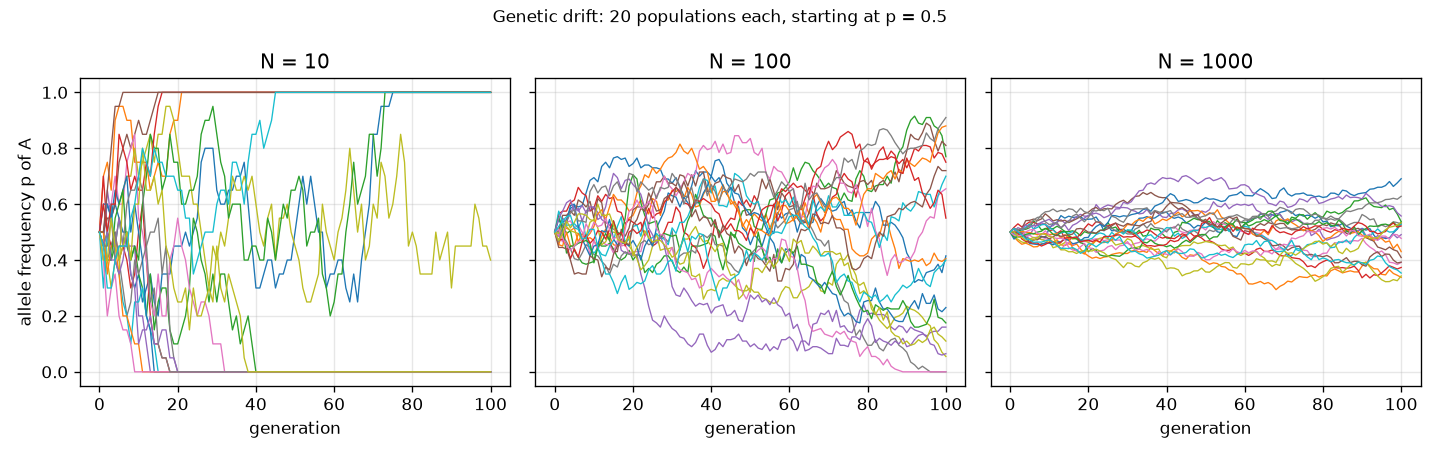
\includegraphics[width=0.85\linewidth]{figures/s03_drift_paths.png}\\\small Twenty populations each at N = 10, 100 and 1000, starting at p = 0.5: smaller populations drift faster.\end{center}

\subsection*{E. Worked example}
(a) With s = 0.10 haploid-like selection and p = 0.10, find p' after one generation. (b) For N = 20 and p\_0 = 0.5, find the expected heterozygosity after 20 generations of drift, and check it with the simulation.
\begin{enumerate}[nosep]
\item (a) p' = p (1 + s) / (1 + s p) = 0.10 x 1.10 / (1 + 0.01) = 0.11 / 1.01 = 0.1089.
\item (b) H\_0 = 2 x 0.5 x 0.5 = 0.5. The factor per generation is 1 - 1/40 = 0.975.
\item After 20 generations: 0.5 x 0.975\textasciicircum{}20 = 0.5 x 0.6027 = 0.3013.
\item Simulation: average 2pq over 20000 seeded populations after 20 generations; it gives 0.3016.
\item The two agree to three decimal places, as expected for a large number of runs.
\end{enumerate}
\textbf{Answer.} (a) p' = 0.1089. (b) Expected heterozygosity 0.3013 against a simulated 0.3016: drift has removed about 40 percent of the variety in 20 generations at N = 20.

\subsection*{F. Questions}
\begin{enumerate}[nosep]
\item \textbf{Conceptual.} A helpful allele is lost in a very small population even though selection favours it. Does this mean selection did not work? Explain.
\item \textbf{Numerical.} A population has N = 50 and a neutral allele. What fraction of heterozygosity is expected after 10 generations? Check the units and sanity.
\item \textbf{Graph and simulation interpretation.} In the N = 10 and N = 5000 panels of the selection figure, what do the grey paths and the dashed curve tell you? What is the spread of p after 20 generations at N = 10 and N = 1000?
\item \textbf{Design and optimisation challenge.} Design: what is the smallest N (diploid individuals) that keeps at least 90 percent of the heterozygosity for 50 generations, and how could you check it? Name two reasons the real number would be larger.
\end{enumerate}

\section{Real-world mini-project}
\textbf{How large must a conservation population be?.} A small captive population is managed to keep its genetic variety. Using the Wright-Fisher model of Session 3 (constant size, random mating, no selection, no migration, no mutation), find the smallest population size N (diploid individuals) that keeps at least 90 percent of the starting heterozygosity for 50 generations. This is a classroom model: real conservation planning uses effective population sizes, sex ratios and many more facts.

\section{The path ahead}
\begin{enumerate}[nosep]
\item \textbf{Session 4: Selfing and inbreeding.} A simulator of repeated selfing starting from one Aa individual.
\item \textbf{Session 5: Unequal sex ratio and effective size.} A Wright-Fisher model with separate sexes.
\item \textbf{Session 6: Linked genes and recombination.} A two-gene gamete simulator with a recombination fraction.
\item \textbf{Session 7: Heterozygote advantage.} Selection with fitness AA 0.8, Aa 1, aa 0.6 and drift in a large population.
\item \textbf{Session 8: Reproduce the Target.} A three-panel animation like the Target, from your own code.
\end{enumerate}

\section{Answers and hints}

\subsection*{Session 1}
\begin{enumerate}[nosep]
\item \textbf{Conceptual.} Hint: A recessive child is aa, so it received an a from each parent. Solution: The child is aa, so each parent passed on an a. A parent who shows the dominant trait must also carry an A, so each parent is Aa. Both parents are carriers of the recessive allele without showing it.
\item \textbf{Numerical.} Hint: Parent 1 can pass only A. Parent 2 passes A or a. Solution: The four boxes are AA, Aa, AA, Aa, so AA : Aa : aa = 2 : 2 : 0. Every child has at least one A, so the chance of the recessive appearance is 0. Sanity check: the four counts add up to 4.
\item \textbf{Graph and simulation interpretation.} Hint: Think about how much one child changes a fraction when the family is small and large. Solution: With 10 children one child changes the fraction by 0.1, so it is easy to land far from 1/4 by chance. With 10000 children one child changes it by 0.0001, and the random ups and downs average out. The Punnett square gives the probability for each child, not the exact count for a small family.
\item \textbf{Design and optimisation challenge.} Hint: Test the three possible pairings that include a recessive parent, and use the square. Solution: Choose Aa x aa: the boxes are Aa, aa, Aa, aa, so half the children are aa (a 1 : 1 ratio). AA x aa gives no recessive children (all Aa) and aa x aa gives only recessive children. Aa x Aa gives only a quarter. Trade-off and assumption: a real cross also needs enough offspring (a small number varies a lot) and a trait that really follows simple dominance.
\end{enumerate}

\subsection*{Session 2}
\begin{enumerate}[nosep]
\item \textbf{Conceptual.} Hint: Compare 2pq with q\textasciicircum{}2 when q is small. Solution: When q is small, q\textasciicircum{}2 is much smaller than 2pq (with q = 0.01, q\textasciicircum{}2 = 0.0001 and 2pq = 0.0198). The allele is rarely paired with another copy of itself, so nearly all copies are in Aa individuals, hidden from view.
\item \textbf{Numerical.} Hint: q = sqrt(1/2500); carriers 2pq. Solution: q = sqrt(0.0004) = 0.02, p = 0.98, carriers = 2 x 0.98 x 0.02 = 0.0392 (about 1 in 26). Sanity check: carriers are roughly 2q = 0.04 when q is small, and 0.0392 is close to that.
\item \textbf{Graph and simulation interpretation.} Hint: Read where the curve crosses the red line, and ask what the expected count is. Solution: From 17 to 33 recessive children the statistic stays below 3.84. The minimum is at 25 because the expected recessive count is 0.25 x 100 = 25, where observed equals expected and chi-square is 0. Both sides rise because larger mismatches are squared.
\item \textbf{Design and optimisation challenge.} Hint: Expected counts are 750 and 250. Use chi-square with the 3.84 limit; the same method gave 17 to 33 for 100 children. Solution: chi-square = (740 - 750)\textasciicircum{}2 / 750 + (260 - 250)\textasciicircum{}2 / 250 = 0.133 + 0.400 = 0.533, below 3.84, so 3:1 is not rejected. For 1000 children the accepted recessive counts are 224 to 276, a band of 53 values (about 22 percent to 28 percent), narrower in relative terms than 17 to 33 percent for 100 children, so a larger sample can detect smaller departures. Assumptions: independent offspring and a simple one-gene model; not rejecting 3:1 does not prove it.
\end{enumerate}

\subsection*{Session 3}
\begin{enumerate}[nosep]
\item \textbf{Conceptual.} Hint: Compare the size of the selection push with the random drift each generation. Solution: Selection still pushes the expected frequency up, but when N is tiny the random drift per generation is much larger than the push, so chance dominates and the allele is often lost early, after which selection cannot bring it back. Selection works on average; drift decides individual cases when N is small. In the simulation the same s = 0.05 allele is lost in about 93 percent of runs at N = 10 and never lost at N = 5000.
\item \textbf{Numerical.} Hint: Multiply the per-generation factor (1 - 1/(2N)) ten times. Solution: The factor is 1 - 1/100 = 0.99, and 0.99\textasciicircum{}10 = 0.9044, so about 90 percent is kept (about 10 percent is lost). H is a pure number with no unit. Sanity check: ten generations at a loss of 1 percent each should lose about 10 percent, and it does.
\item \textbf{Graph and simulation interpretation.} Hint: Compare how closely the paths follow the dashed curve, and read the spread from the drift figure. Solution: At N = 5000 the paths hug the deterministic curve, so selection is nearly predictable. At N = 10 the paths scatter and most end at 0, so drift can overrule selection. The spread (standard deviation) of p after 20 generations starting at 0.5 is about 0.4 at N = 10 and about 0.05 at N = 1000, which is why larger populations are more predictable.
\item \textbf{Design and optimisation challenge.} Hint: Solve (1 - 1/(2N))\textasciicircum{}50 \textgreater{}= 0.9, using ln, then check integers near the answer. Solution: Taking logs: 50 ln(1 - 1/(2N)) \textgreater{}= ln 0.9, so 1 - 1/(2N) \textgreater{}= 0.9\textasciicircum{}(1/50) = 0.997895, which gives N \textgreater{}= 237.5, so N = 238. Check: N = 238 gives 0.9002 and N = 237 gives 0.8998. A simulation at N = 238 with 5000 seeded runs keeps about 0.90 of H (0.898 in the checkpoint). The real number would be larger because the effective size is smaller than the head count (unequal sex ratio, uneven family sizes), and because mutation and migration are ignored while the target may be stricter than 90 percent.
\end{enumerate}

\section{How to join}
Read \texttt{CONTRIBUTING.md} in the repository, then pick an issue labelled \texttt{good first issue}. Repository: \url{https://github.com/KrunalPanchal1995/opengenetics}

\end{document}
